\subsection{FET}
Al igual que con el BJT, el propósito de la polarización es seleccionar el
voltaje de cd de compuerta a fuente apropiado para establecer un valor deseado
de la corriente en el drenaje y, por consiguiente, un punto Q apropiado
\cite{Floyd}.

\subsubsection{Divisor de voltaje}
La configuración del divisor de voltaje aplicada a amplificadores con
transistores BJT también se aplica a amplificadores con FET como se muestra en
la \textbf{figura~\ref{figura14}}. La construcción básica es exactamente la misma,
pero el análisis de cada una es muy diferente.

\begin{figure}[!ht]
\centering
\includegraphics[scale=0.26]{diagramas/figura14.eps}
\caption{Circuito divisor de voltaje.}
\label{figura14}
\end{figure}

Una curva de transferencia para un \textbf{JFET} se expresa aproximadamente
como:
\begin{equation*}
    I_{\text{D}} \cong I_{\text{DSS}}
    \left(1-\frac{V_{\text{GS}}}{V_{\text{GS(corte)}}}\right)^2
\end{equation*}

La recta de carga de CD con divisor de voltaje se determina de la siguiente
manera:

Con $I_\text{D} = 0$:
\begin{equation*}
    \begin{split}
        V_\text{S} &= I_{\text{D}}\,R_{\text{S}}
                   = (0)\,R_{\text{S}}
                   = 0[V]\\
        V_\text{GS} &= V_{\text{G}} - V_{\text{S}}
                    = V_{\text{G}} - 0[V]
                    = V_{\text{G}}\\
    \end{split}
\end{equation*}

Donde $V_{\text{G}}$:
\begin{equation*}
    V_{\text{G}} = \left(\frac{R_2}{R_1+R_2}\right)\,V_{\text{DD}}
\end{equation*}

Por consiguiente, un punto sobre la recta está en $I_{\text{D}} = 0$ y
$V_{\text{GS}} = V_{\text{G}}$.

Con $V_{\text{GS}} = 0$:
\begin{equation*}
    I_\text{D} = \frac{V_{\text{G}} - V_{\text{GS}}}{R_{\text{S}}}
               = \frac{V_{\text{G}}}{R_{\text{S}}}
\end{equation*}

El punto donde la recta de carga corta la curva de transferencia es el punto
$Q$ \cite{Floyd}.
\begin{equation*}
    \left(\frac{I_{\text{DSS}}}{V_{\text{GS(corte)}}^2}\right)\,
    V_{\text{GS}}^2 + \left(\frac{1}{R_{\text{S}}}-
    \frac{2\,I_{\text{DSS}}}{V_{\text{GS(corte)}}}\right)\,
    V_{\text{GS}}+
    \left(I_{\text{DSS}}-\frac{V_{\text{G}}}{R_{\text{S}}}\right) = 0
\end{equation*}

Resolviendo la ecuación cuadrática es posible encontrar el punto $Q$ del
circuito.

\subsubsection{Criterios de diseño}
Normalmente es deseable polarizar un JFET cerca del punto medio de su curva de
transferencia donde $I_{\text{D}} = I_{\text{DSS}}/2$. En condiciones de señal,
la polarización en el punto medio permite que la cantidad máxima de corriente en
el drenaje oscile entre $I_{\text{DSS}}$ y $0$ \cite{Floyd}.
\begin{equation*}
    \begin{split}
        I_{\text{D}} &\rightarrow 0.5\,I_{\text{DSS}}\\
        V_{\text{G}} &\rightarrow 0.5\,V_{\text{GS(corte)}}\\
    \end{split}
\end{equation*}

De la misma manera que en la polarización BJT, también se considerará que el
voltaje entre el drenaje y fuente se encuentre en el punto medio del voltaje de
alimentación:
\begin{equation*}
    V_{\text{GS}} = \frac{1}{2}\,V_{\text{DD}}
\end{equation*}

Nótese que no se necesita colocar el punto Q en el centro de la linea de carga
de ca como se hizo para la polarización del BJT; esto se debe a que normalmente
se utiliza un amplificador FET en la entrada del amplificador para sacar ventaja
de la alta resistencia de entrada. En este punto, los niveles de tensión son tan
pequeños que no se excita al amplificador con grades excursiones. Además, como
las curvas características no son lineales, se produciría distorsión con grandes
excursiones de entrada \cite{Savant}.

Se considerara usar el conjunto de valores cuyo $V_{\text{DS}}$ sea el mas alto
posible:
\begin{equation*}
    V_{\text{DS}} = V_{\text{DD}} - I_{\text{D}}\,(R_{\text{D}} + R_{\text{S}})
\end{equation*}

También se deben considerar las potencias disipadas máximas por las
resistencias:
\begin{equation*}
    \{P_{R_1}, P_{R_2}, P_{R_D}, P_{R_S}\} < 0.2[\text{W}]\\
\end{equation*}

\subsubsection{Voltaje de alimentación}
Para el diseño del amplificador se seleccionó un voltaje de alimentación de
$9\,[\text{V}]$.
\begin{equation*}
    V_{\text{CC}} = 9\,[\text{V}]
\end{equation*}

\subsubsection{Resistencias disponibles}
Se cuenta con una serie de resistencias de $0.5[\text{W}]$ con los valores
detallados en el \textbf{cuadro~\ref{cuadro06}}.

\subsubsection{Calculo computarizado}
Una vez descritos los criterios de diseño y las formulas para el calculo de las
resistencias del divisor de voltaje, se ha escrito un programa para el software
matemático \emph{Octave}, que permute todas las combinaciones posibles de las 
resistencia e imprima aquellas que cumplen todos los criterios.

\scriptsize
\begin{shaded}
\begin{verbatim}
% polarizacion por divisor de voltaje (2N3819 canal n)
Vdd = 9;            % [V]
Idss = 15.8e-3;     % [A]
Vgso = -1.037;      % [V]

% resistencias disponibles
R = [
    1 ...
    10            22             47 ...
    100 150 200   220 270 330    470   510    680 ...
    1000    2000  2200    3300   4700  5100   6800 ...
    10000   20000                47000 51000  68000 ...
    100000        220000  330000       510000 ...
    1000000
];

count = 1;
printf(' ,R1[Ω],R2[Ω],Rd[Ω],Rs[Ω] -> Vg[V]\t\tId[mA] Vds[V],P1[mW],P2[mW],Pd[mW],Ps[mW]\n');

for (h = 1:length(R))
    for (i = 1:length(R))
        for (j = 1:length(R))
            for (k = 1:length(R))
                R1 = R(h);
                R2 = R(i);
                Rd = R(j);
                Rs = R(k);

                Vg = (R2 / (R1 + R2)) * Vdd;    % Id = 0
                Id = Vg / Rs;                   % Vgs = 0

                QVg = roots([Idss/(Vgso^2), (1/Rs) - (2*(Idss/Vgso)), Idss-Id]);
                QId = (-1/Rs) * (QVg(2) - Vg);

                P1 = ((Vdd - QVg(2))^2) / R1;
                P2 = (QVg(2)^2) / R2;
                Pd = QId^2 * Rd;
                Ps = QId^2 * Rs;

                Vds = Vdd - (QId * (Rd + Rs));

                if(
                    (abs(Vgso - (2 * QVg(2))) < 0.4)&&         % Vg -> Vgs0/2
                    (abs(Idss - (2 * QId)) < 0.00075)&&     % Id -> Idss/2
                    (abs((Vdd / 2) - Vds) < 0.5)&&          % 4.0 < Vds < 5.0[V]
                    (0.001<P1)&&(P1<0.2)&&                  % 0.001 < P1 < 0.2
                    (0.001<P2)&&(P2<0.2)&&                  % 0.001 < P2 < 0.2
                    (0.001<Pd)&&(Pd<0.2)&&                  % 0.001 < Pd < 0.2
                    (0.001<Ps)&&(Ps<0.2)                    % 0.001 < Ps < 0.2
                )
                    printf(
                        '%d,%d,%d,%d,%d -> (%.2f, 0) (0, %.3f) %.2f,%.2f,%.2f,%.2f,%.2f,%.2f,%.2f\n',
                        count,
                        R(h), R(i), R(j), R(k),
                        Vg,Id * 1e3,
                        QVg(2), QId * 1e3,
                        Vds,
                        P1 * 1e3,
                        P2 * 1e3,
                        Pd * 1e3,
                        Ps * 1e3
                    );

                    count++;
                endif
            endfor
        endfor
    endfor
endfor
\end{verbatim}
\end{shaded}
\normalsize

\subsubsection{Resultados del calculo computarizado}
La salida del programa detalla los valores de las cuatro resistencias ($R_1$,
$R_2$, $R_D$, $R_S$), los valores de potencia en cada una de las resistencias
($P_1$, $P_2$, $P_D$, $P_S$), estos valores pueden verse en el
\textbf{cuadro~\ref{cuadro10}}.

\begin{table}[!h]
\begin{center}
    \begin{tabular}{|c|c|c|c||c||c|c|c|c|}
    \hline
    $R_1[\Omega]$ & $R_2[\Omega]$ & $R_D[\Omega]$ & $R_S[\Omega]$ &
    $V_{DS}[V]$ &
    $P_1[mW]$ & $P_2[mW]$ & $P_D[mW]$ & $P_S[mW]$
    \tabularnewline \hline \hline
    $ 470$ & $ 47$ & $470$ & $150$ & $4.30$ & $184.76$ & $2.16$ & $27.0$ & $8.62$ \tabularnewline \hline
    $1000$ & $100$ & $470$ & $150$ & $4.30$ & $ 86.84$ & $1.02$ & $27.0$ & $8.62$ \tabularnewline \hline
    \end{tabular}
\end{center}
\caption{Resultados del calculo computarizado.}
\label{cuadro10}
\end{table}

Mientras que los valores de voltaje de compuerta ($V_{\text{G}}$) y la corriente
de drenaje ($I_D$) son fijos para todos los casos.
\begin{equation*}
    \begin{split}
        V_{\text{G}} &= -0.32[V]\\
        I_{\text{D}} &= 7.58[mA]\\
    \end{split}
\end{equation*}

\subsubsection{Simulación de computadora}
Se utilizó el software \emph{Quite Universal Circuit Simulator.} versión 23.3.1
para simular el circuito, este puede verse en la
\textbf{figura~\ref{figura15}} y los valores calculados en el simulador pueden
verse en el \textbf{cuadro~\ref{cuadro11}}.

\begin{figure}[!h]
\centering
\includegraphics[scale=1.00]{diagramas/figura15.eps}
\caption{Simulación del circuito.}
\label{figura15}
\end{figure}

\begin{table}[!h]
\begin{center}
    \begin{tabular}{|c|c|c|c||c||c|c|}
    \hline
    $R_1[\Omega]$ & $R_2[\Omega]$ & $R_D[\Omega]$ & $R_S[\Omega]$ &
    $V_{\text{DS}}$ & $V_{\text{G}}[V]$ & $I_{\text{D}}[mA]$
    \tabularnewline \hline \hline
    $ 470$ & $ 47$ & $470$ & $150$ & $4.11$ & $-0.364$ & $7.88$ \tabularnewline \hline
    $1000$ & $100$ & $470$ & $150$ & $4.11$ & $-0.364$ & $7.88$ \tabularnewline \hline
    \end{tabular}
\end{center}
\caption{Resultados obtenidos de la simulación.}
\label{cuadro11}
\end{table}

\subsubsection{Placa de prueba}
El circuito armado puede verse en la \textbf{figura~\ref{figura16}}, alimentado
por una fuente estable de $9[\text{V}]$.

En el circuito se fueron variando las resistencias obtenidas en el calculo
anterior, y se midieron los valores de voltaje y corriente, estos se muestran
en el \textbf{cuadro~\ref{cuadro12}}.

\begin{figure}[!h]
\centering
\includegraphics[scale=0.125]{diagramas/figura16.eps}
\caption{Polarización con divisor de voltaje en placa de pruebas.}
\label{figura16}
\end{figure}

\begin{table}[!h]
\begin{center}
    \begin{tabular}{|c|c|c|c||c||c|c|}
    \hline
    $R_1[\Omega]$ & $R_2[\Omega]$ & $R_D[\Omega]$ & $R_S[\Omega]$ &
    $V_{\text{DS}}$ & $V_{\text{G}}[V]$ & $I_{\text{D}}[mA]$
    \tabularnewline \hline \hline
    $ 470$ & $ 47$ & $470$ & $150$ & $4.62$ & $-0.208$ & $7.03$ \tabularnewline \hline
    $1000$ & $100$ & $470$ & $150$ & $4.65$ & $-0.209$ & $7.00$ \tabularnewline \hline
    \end{tabular}
\end{center}
\caption{Valores medidos en la placa de pruebas.}
\label{cuadro12}
\end{table}

\subsubsection{Valores de polarización}
Considerando que todos los valores obtenidos tienen valores similares, se
utilizaran los de menor disipación de potencia. Con lo cual se halla el punto
$Q$ de operación, que puede verse en la \textbf{figura~\ref{curva03}}.

\begin{figure}[!ht]
    \centering
    % GNUPLOT: LaTeX picture with Postscript
\begingroup
  \makeatletter
  \providecommand\color[2][]{%
    \GenericError{(gnuplot) \space\space\space\@spaces}{%
      Package color not loaded in conjunction with
      terminal option `colourtext'%
    }{See the gnuplot documentation for explanation.%
    }{Either use 'blacktext' in gnuplot or load the package
      color.sty in LaTeX.}%
    \renewcommand\color[2][]{}%
  }%
  \providecommand\includegraphics[2][]{%
    \GenericError{(gnuplot) \space\space\space\@spaces}{%
      Package graphicx or graphics not loaded%
    }{See the gnuplot documentation for explanation.%
    }{The gnuplot epslatex terminal needs graphicx.sty or graphics.sty.}%
    \renewcommand\includegraphics[2][]{}%
  }%
  \providecommand\rotatebox[2]{#2}%
  \@ifundefined{ifGPcolor}{%
    \newif\ifGPcolor
    \GPcolorfalse
  }{}%
  \@ifundefined{ifGPblacktext}{%
    \newif\ifGPblacktext
    \GPblacktexttrue
  }{}%
  % define a \g@addto@macro without @ in the name:
  \let\gplgaddtomacro\g@addto@macro
  % define empty templates for all commands taking text:
  \gdef\gplbacktext{}%
  \gdef\gplfronttext{}%
  \makeatother
  \ifGPblacktext
    % no textcolor at all
    \def\colorrgb#1{}%
    \def\colorgray#1{}%
  \else
    % gray or color?
    \ifGPcolor
      \def\colorrgb#1{\color[rgb]{#1}}%
      \def\colorgray#1{\color[gray]{#1}}%
      \expandafter\def\csname LTw\endcsname{\color{white}}%
      \expandafter\def\csname LTb\endcsname{\color{black}}%
      \expandafter\def\csname LTa\endcsname{\color{black}}%
      \expandafter\def\csname LT0\endcsname{\color[rgb]{1,0,0}}%
      \expandafter\def\csname LT1\endcsname{\color[rgb]{0,1,0}}%
      \expandafter\def\csname LT2\endcsname{\color[rgb]{0,0,1}}%
      \expandafter\def\csname LT3\endcsname{\color[rgb]{1,0,1}}%
      \expandafter\def\csname LT4\endcsname{\color[rgb]{0,1,1}}%
      \expandafter\def\csname LT5\endcsname{\color[rgb]{1,1,0}}%
      \expandafter\def\csname LT6\endcsname{\color[rgb]{0,0,0}}%
      \expandafter\def\csname LT7\endcsname{\color[rgb]{1,0.3,0}}%
      \expandafter\def\csname LT8\endcsname{\color[rgb]{0.5,0.5,0.5}}%
    \else
      % gray
      \def\colorrgb#1{\color{black}}%
      \def\colorgray#1{\color[gray]{#1}}%
      \expandafter\def\csname LTw\endcsname{\color{white}}%
      \expandafter\def\csname LTb\endcsname{\color{black}}%
      \expandafter\def\csname LTa\endcsname{\color{black}}%
      \expandafter\def\csname LT0\endcsname{\color{black}}%
      \expandafter\def\csname LT1\endcsname{\color{black}}%
      \expandafter\def\csname LT2\endcsname{\color{black}}%
      \expandafter\def\csname LT3\endcsname{\color{black}}%
      \expandafter\def\csname LT4\endcsname{\color{black}}%
      \expandafter\def\csname LT5\endcsname{\color{black}}%
      \expandafter\def\csname LT6\endcsname{\color{black}}%
      \expandafter\def\csname LT7\endcsname{\color{black}}%
      \expandafter\def\csname LT8\endcsname{\color{black}}%
    \fi
  \fi
    \setlength{\unitlength}{0.0500bp}%
    \ifx\gptboxheight\undefined%
      \newlength{\gptboxheight}%
      \newlength{\gptboxwidth}%
      \newsavebox{\gptboxtext}%
    \fi%
    \setlength{\fboxrule}{0.5pt}%
    \setlength{\fboxsep}{1pt}%
    \definecolor{tbcol}{rgb}{1,1,1}%
\begin{picture}(6480.00,4030.00)%
    \gplgaddtomacro\gplbacktext{%
      \csname LTb\endcsname%%
      \put(3190,440){\makebox(0,0)[r]{\strut{}}}%
      \csname LTb\endcsname%%
      \put(3190,864){\makebox(0,0)[r]{\strut{}}}%
      \csname LTb\endcsname%%
      \put(3190,1287){\makebox(0,0)[r]{\strut{}}}%
      \csname LTb\endcsname%%
      \put(3190,1711){\makebox(0,0)[r]{\strut{}}}%
      \csname LTb\endcsname%%
      \put(3190,2135){\makebox(0,0)[r]{\strut{}}}%
      \csname LTb\endcsname%%
      \put(3190,2558){\makebox(0,0)[r]{\strut{}}}%
      \csname LTb\endcsname%%
      \put(3190,2982){\makebox(0,0)[r]{\strut{}}}%
      \csname LTb\endcsname%%
      \put(3190,3405){\makebox(0,0)[r]{\strut{}}}%
      \csname LTb\endcsname%%
      \put(3190,3829){\makebox(0,0)[r]{\strut{}}}%
      \csname LTb\endcsname%%
      \put(755,240){\makebox(0,0){\strut{}}}%
      \csname LTb\endcsname%%
      \put(2032,240){\makebox(0,0){\strut{}}}%
      \csname LTb\endcsname%%
      \put(3310,240){\makebox(0,0){\strut{}}}%
      \csname LTb\endcsname%%
      \put(4587,240){\makebox(0,0){\strut{}}}%
      \csname LTb\endcsname%%
      \put(5864,240){\makebox(0,0){\strut{}}}%
      \csname LTb\endcsname%%
      \put(500,228){\makebox(0,0)[l]{\strut{}-1.04}}%
      \put(1981,652){\makebox(0,0)[l]{\strut{}-0.32}}%
      \put(2850,652){\makebox(0,0)[l]{\strut{}-0.21}}%
      \put(5225,228){\makebox(0,0)[l]{\strut{}0.82}}%
      \put(3565,1594){\makebox(0,0)[l]{\strut{}5.46}}%
      \put(3565,1902){\makebox(0,0)[l]{\strut{}7.0}}%
      \put(3565,2135){\makebox(0,0)[l]{\strut{}7.58}}%
      \put(3565,3617){\makebox(0,0)[l]{\strut{}15.8}}%
    }%
    \gplgaddtomacro\gplfronttext{%
      \csname LTb\endcsname%%
      \put(190,2134){\rotatebox{-270.00}{\makebox(0,0){\strut{}$I_{\text{D}}[mA]$}}}%
      \put(3309,140){\makebox(0,0){\strut{}$V_{\text{GS}}[V]$}}%
    }%
    \gplgaddtomacro\gplbacktext{%
      \csname LTb\endcsname%%
      \put(3190,440){\makebox(0,0)[r]{\strut{}}}%
      \csname LTb\endcsname%%
      \put(3190,864){\makebox(0,0)[r]{\strut{}}}%
      \csname LTb\endcsname%%
      \put(3190,1287){\makebox(0,0)[r]{\strut{}}}%
      \csname LTb\endcsname%%
      \put(3190,1711){\makebox(0,0)[r]{\strut{}}}%
      \csname LTb\endcsname%%
      \put(3190,2135){\makebox(0,0)[r]{\strut{}}}%
      \csname LTb\endcsname%%
      \put(3190,2558){\makebox(0,0)[r]{\strut{}}}%
      \csname LTb\endcsname%%
      \put(3190,2982){\makebox(0,0)[r]{\strut{}}}%
      \csname LTb\endcsname%%
      \put(3190,3405){\makebox(0,0)[r]{\strut{}}}%
      \csname LTb\endcsname%%
      \put(3190,3829){\makebox(0,0)[r]{\strut{}}}%
      \csname LTb\endcsname%%
      \put(755,240){\makebox(0,0){\strut{}}}%
      \csname LTb\endcsname%%
      \put(2032,240){\makebox(0,0){\strut{}}}%
      \csname LTb\endcsname%%
      \put(3310,240){\makebox(0,0){\strut{}}}%
      \csname LTb\endcsname%%
      \put(4587,240){\makebox(0,0){\strut{}}}%
      \csname LTb\endcsname%%
      \put(5864,240){\makebox(0,0){\strut{}}}%
      \csname LTb\endcsname%%
      \put(500,228){\makebox(0,0)[l]{\strut{}-1.04}}%
      \put(1981,652){\makebox(0,0)[l]{\strut{}-0.32}}%
      \put(2850,652){\makebox(0,0)[l]{\strut{}-0.21}}%
      \put(5225,228){\makebox(0,0)[l]{\strut{}0.82}}%
      \put(3565,1594){\makebox(0,0)[l]{\strut{}5.46}}%
      \put(3565,1902){\makebox(0,0)[l]{\strut{}7.0}}%
      \put(3565,2135){\makebox(0,0)[l]{\strut{}7.58}}%
      \put(3565,3617){\makebox(0,0)[l]{\strut{}15.8}}%
    }%
    \gplgaddtomacro\gplfronttext{%
      \csname LTb\endcsname%%
      \put(190,2134){\rotatebox{-270.00}{\makebox(0,0){\strut{}$I_{\text{D}}[mA]$}}}%
      \put(3309,140){\makebox(0,0){\strut{}$V_{\text{GS}}[V]$}}%
    }%
    \gplbacktext
    \put(0,0){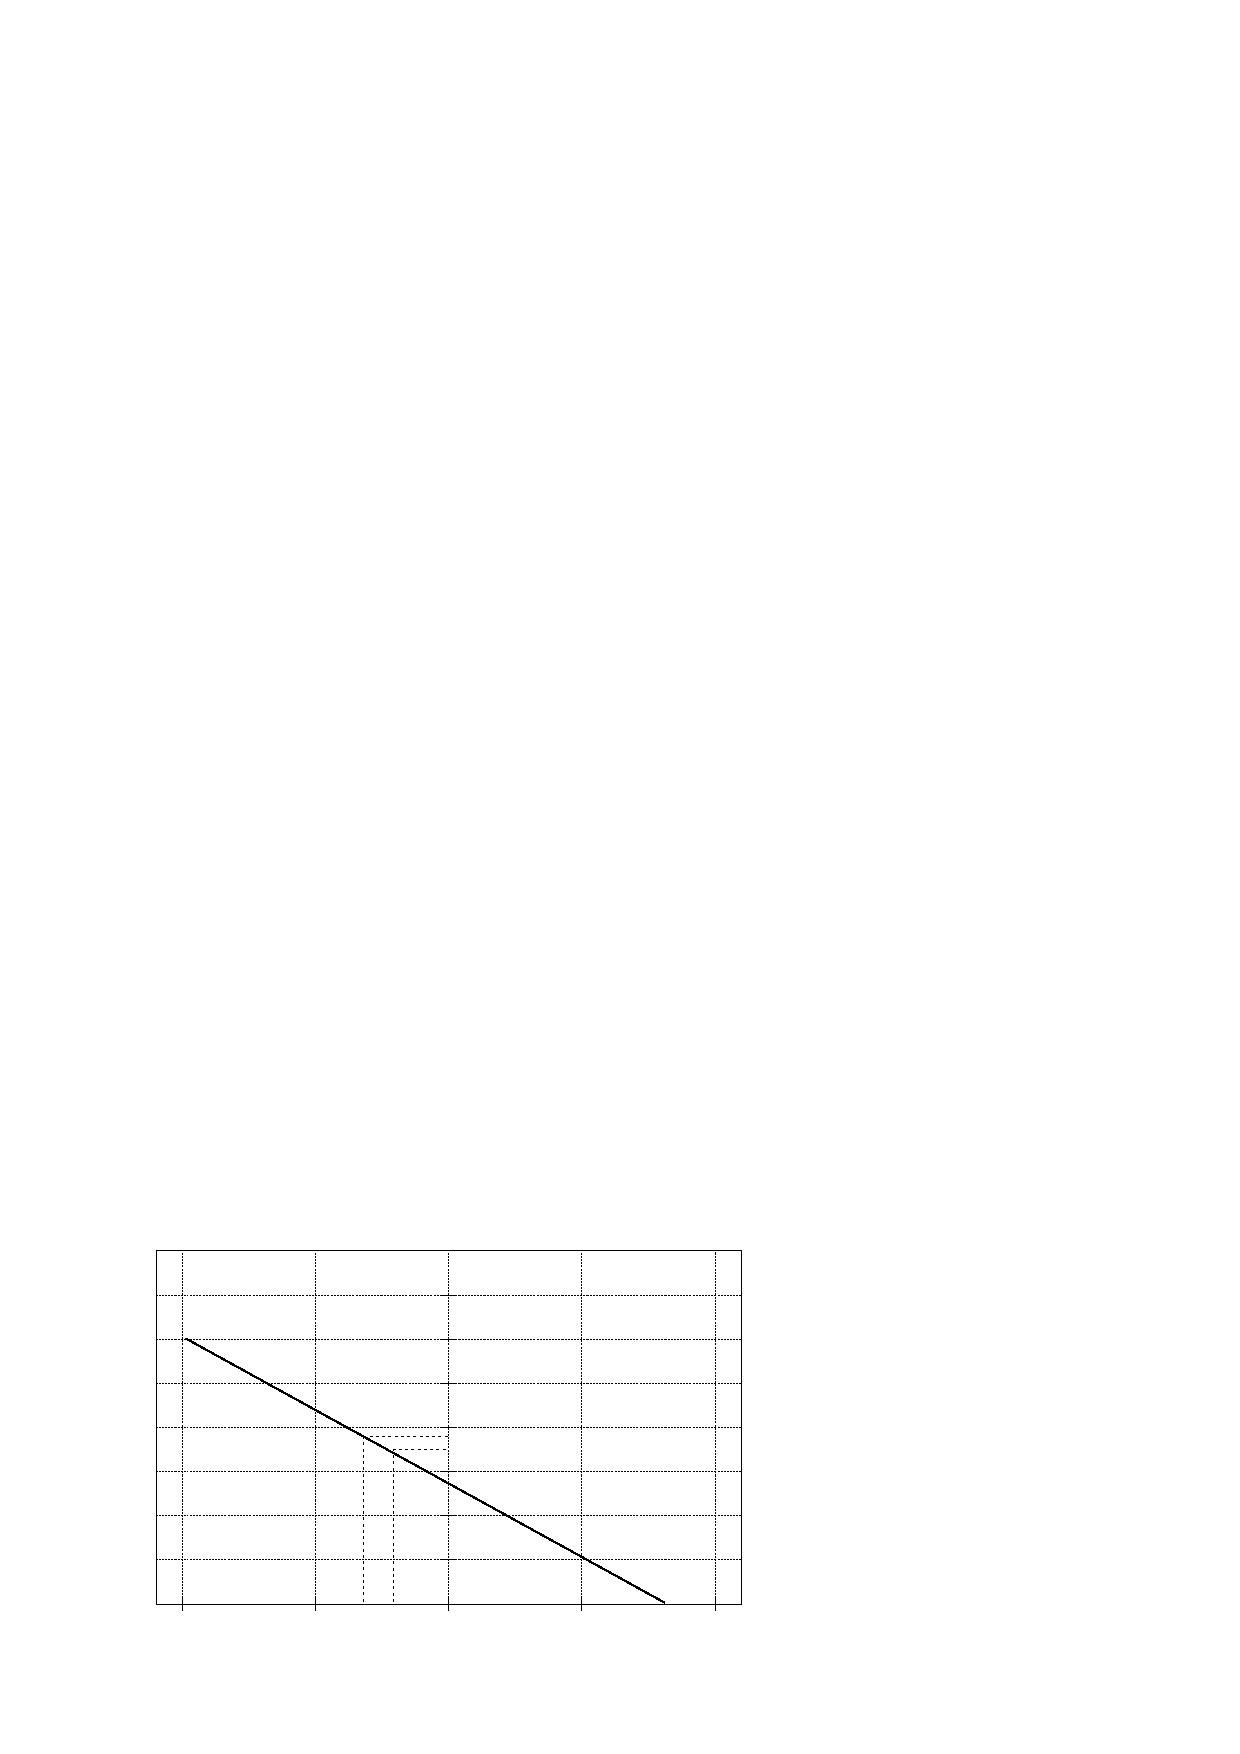
\includegraphics[width={324.00bp},height={201.50bp}]{curva3}}%
    \gplfronttext
  \end{picture}%
\endgroup

    \caption{Punto $Q$ hallado.}
    \label{curva03}
\end{figure}

Según las pruebas realizadas los valores obtenidos son:
\begin{equation*}
    \begin{split}
        R_{\text{1}} &= 1[k\Omega]\\
        R_{\text{2}} &= 100[\Omega]\\
        R_{\text{D}} &= 470[\Omega]\\
        R_{\text{S}} &= 150[\Omega]\\
\end{split}
\end{equation*}

Punto $Q$:
\begin{equation*}
    \begin{split}
        V_{\text{GS}} = -0.209\,[\text{V}]\\
        I_{\text{D}} = 7.0\,[\text{mA}]\\
    \end{split}
\end{equation*}

Rango máximo de voltaje de compuerta: 
$-0.42[{\text{V}}] < V_{\text{GS}} < 0[{\text{V}}]$.

